\documentclass[border=2pt,multi=tikzpicture]{standalone}
\usepackage{tikz}
\usetikzlibrary{positioning, arrows.meta, calc}
\newcommand{\cnum}[1]{\textbf{\textcircled{\raisebox{-0.4pt}{\tiny #1}}}}
\tikzset{
  arr/.style={-{Latex[length=1.8mm,width=1.5mm]}, semithick, draw=black!80},
  barr/.style={-{Latex[length=1.8mm,width=1.5mm]}, semithick, draw=black!80, densely dashed},
  blk/.style={draw=black!65, rounded corners=1.4pt, align=center, inner sep=2.8pt, fill=white},
  lab/.style={font=\tiny, align=center, inner sep=1.2pt, fill=white}
}
\begin{document}
% =========== FIG A: where positions come from ===========
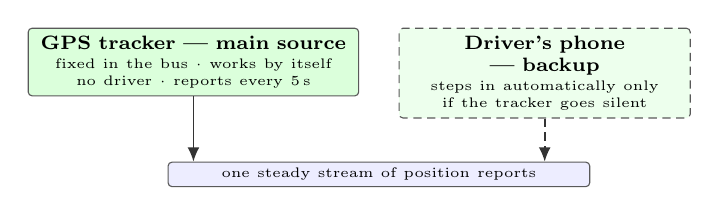
\begin{tikzpicture}[font=\scriptsize]
\node[blk, fill=green!14, text width=40mm] (gt)
  {\textbf{GPS tracker --- main source}\\[-1pt]
   {\tiny fixed in the bus $\cdot$ works by itself}\\[-2pt]
   {\tiny no driver $\cdot$ reports every 5\,s}};
\node[blk, fill=green!7, densely dashed, text width=35mm, anchor=north west]
  (ph) at ($(gt.north east)+(5mm,0)$)
  {\textbf{Driver's phone --- backup}\\[-1pt]
   {\tiny steps in automatically only}\\[-2pt]
   {\tiny if the tracker goes silent}};
\node[blk, fill=blue!7, text width=52mm, inner sep=2.2pt] (out)
  at ($(gt.south east)!0.5!(ph.south west)+(0,-8.5mm)$)
  {\tiny one steady stream of position reports};
\draw[arr]  (gt.south) -- (gt.south |- out.north);
\draw[barr] (ph.south) -- (ph.south |- out.north);
\end{tikzpicture}
% =========== FIG B: how reports reach the server ===========
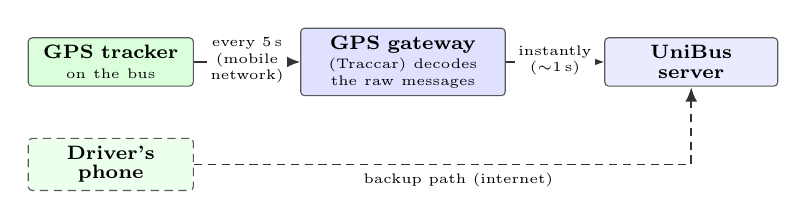
\begin{tikzpicture}[font=\scriptsize]
\node[blk, fill=green!14, text width=19mm] (gt)
  {\textbf{GPS tracker}\\[-1pt]{\tiny on the bus}};
\node[blk, fill=blue!12, text width=24mm, right=13.5mm of gt] (trac)
  {\textbf{GPS gateway}\\[-1pt]{\tiny (Traccar) decodes}\\[-2pt]{\tiny the raw messages}};
\node[blk, fill=blue!8, text width=20mm, right=12.5mm of trac] (app)
  {\textbf{UniBus}\\[-1pt]\textbf{server}};
\node[blk, fill=green!7, densely dashed, text width=19mm, below=6.5mm of gt] (ph)
  {\textbf{Driver's}\\[-1pt]\textbf{phone}};
\draw[arr] (gt) -- (trac)
  node[lab, midway, yshift=0.2mm] {every 5\,s\\(mobile\\network)};
\draw[arr] (trac) -- (app)
  node[lab, midway, yshift=0.2mm] {instantly\\($\sim$1\,s)};
\draw[barr] (ph.east) -- ++(4mm,0) -| ($(app.south)+(0,-0.1mm)$)
  node[lab, pos=0.25, anchor=north, yshift=-0.6mm] {backup path (internet)};
\end{tikzpicture}
% =========== FIG C: what the server does ===========
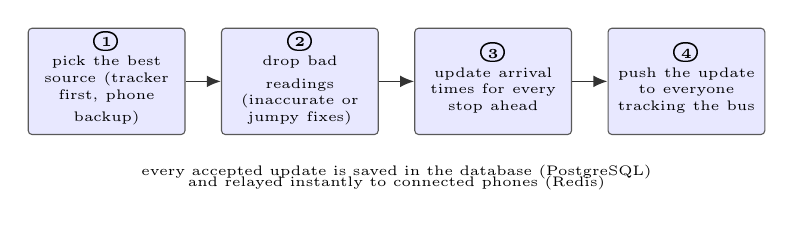
\begin{tikzpicture}[font=\scriptsize,
  st/.style={blk, fill=blue!9, text width=18.5mm, inner sep=2pt, minimum height=13.5mm}]
\node[st] (a) {\cnum{1}\\[-1pt]{\tiny pick the best}\\[-2pt]{\tiny source (tracker}\\[-2pt]{\tiny first, phone backup)}};
\node[st, right=4.5mm of a] (b) {\cnum{2}\\[-1pt]{\tiny drop bad readings}\\[-2pt]{\tiny (inaccurate or}\\[-2pt]{\tiny jumpy fixes)}};
\node[st, right=4.5mm of b] (c) {\cnum{3}\\[-1pt]{\tiny update arrival}\\[-2pt]{\tiny times for every}\\[-2pt]{\tiny stop ahead}};
\node[st, right=4.5mm of c] (d) {\cnum{4}\\[-1pt]{\tiny push the update}\\[-2pt]{\tiny to everyone}\\[-2pt]{\tiny tracking the bus}};
\draw[arr] (a) -- (b); \draw[arr] (b) -- (c); \draw[arr] (c) -- (d);
\node[font=\tiny, align=center, below=2.6mm of $(b.south)!0.5!(c.south)$]
  {every accepted update is saved in the database (PostgreSQL)\\[-2pt]
   and relayed instantly to connected phones (Redis)};
\end{tikzpicture}
% =========== FIG D: who sees the result ===========
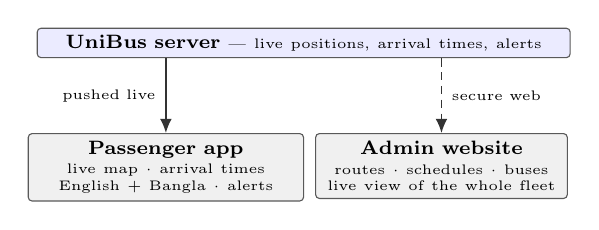
\begin{tikzpicture}[font=\scriptsize]
\node[blk, fill=blue!8, text width=66mm, inner sep=2.4pt] (app)
  {\textbf{UniBus server} {\tiny --- live positions, arrival times, alerts}};
\node[blk, fill=black!6, text width=33mm, anchor=north]
  (pass) at ($(app.south)+(-17.5mm,-9.5mm)$)
  {\textbf{Passenger app}\\[-1pt]
   {\tiny live map $\cdot$ arrival times}\\[-2pt]
   {\tiny English $+$ Bangla $\cdot$ alerts}};
\node[blk, fill=black!6, text width=30mm, anchor=north]
  (adm) at ($(app.south)+(17.5mm,-9.5mm)$)
  {\textbf{Admin website}\\[-1pt]
   {\tiny routes $\cdot$ schedules $\cdot$ buses}\\[-2pt]
   {\tiny live view of the whole fleet}};
\draw[arr] ($(app.south)+(-17.5mm,0)$) -- (pass.north)
  node[lab, midway, anchor=east, xshift=-0.8mm] {pushed live};
\draw[barr] ($(app.south)+(17.5mm,0)$) -- (adm.north)
  node[lab, midway, anchor=west, xshift=0.8mm] {secure web};
\end{tikzpicture}
\end{document}
